Модель достигла неплохого качества в задаче классификации: ROC-AUC=0.9, accuracy=0.82. Попробуем интерпретировать ее результаты.

Нулевой способ это встроенный метод XGBoost, показывающий важность признаков при предсказании. Посмотрим на первые 5 самых важных признаков. Данная величина может быть расчитана тремя способами: <<weight>>, <<gain>>, <<cover>>. Первый показывает, сколько раз признак появляется в дереве:

\begin{figure}[h]
	\centering{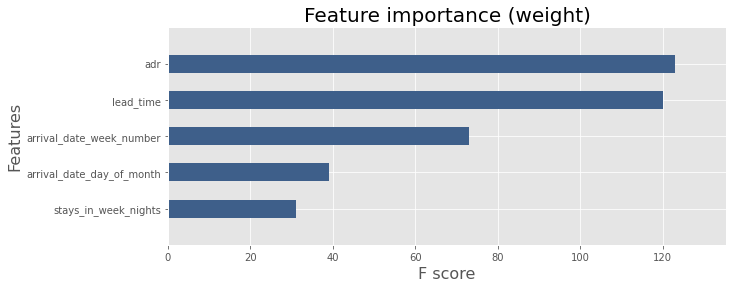
\includegraphics[width=0.85\linewidth]{pics/imp1.png}}
\end{figure}

Второй -- на сколько в среднем уменьшалась ошибка при использовании данного признака:

\begin{figure}[h]
	\centering{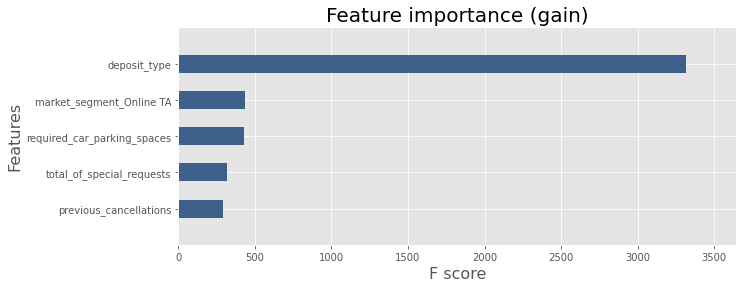
\includegraphics[width=0.85\linewidth]{pics/imp2.png}}
\end{figure}

И последний -- какое количество объектов выборки задействовало узлы с заданным признаком:

\begin{figure}[h]
	\centering{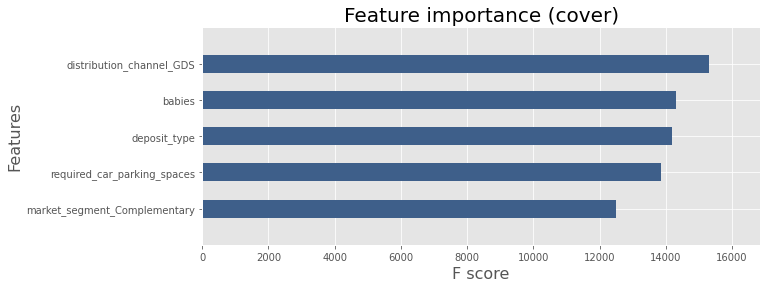
\includegraphics[width=0.85\linewidth]{pics/imp3.png}}
\end{figure}

Теперь перейдем к описанным ранее методам. Первый -- PDP. Возьмем признаки, которые сам XGBoost посчитал наиболее важными: первые два из weight (adr, lead\_time), первый из gain (deposit\_type) и первый из cover (distribution\_channel\_GDS) -- они с отрывом вырываются в лидеры.

И также возьмем признаки, которые XGBoost счел самыми незначительными: последний из weight (distribution\_channel\_GDS, забавно -- в тренировочной выборке всего 145 объектов, которым соответствует GDS. Судя по всему данный признак встречается 1-2 раза в узлах деревьев, но при этом он отсекает очень много объектов, из-за чего cover считает его важным), последний из gain (customer\_type\_group) и последний из cover (market\_segment\_Offline TA/TO).

Построим для них PDP.

\begin{tabular}{c|c}
	\arrayrulecolor[rgb]{0.8,0.85,1}
	\includegraphics*[width = 0.47\textwidth]{pics/mypdp1.png} & \includegraphics*[width = 0.47\textwidth]{pics/mypdp2.png}\\
	\hline
	\includegraphics*[width = 0.47\textwidth]{pics/mypdp3.png} & \includegraphics*[width = 0.47\textwidth]{pics/mypdp4.png}\\
	\hline
	\includegraphics*[width = 0.47\textwidth]{pics/mypdp5.png} & \includegraphics*[width = 0.47\textwidth]{pics/mypdp6.png}\\
\end{tabular}\\[2mm]

Первый признак является непрерывным, второй --  дискретным, третий -- порядковым, остальные -- бинарными. Для первых двух видно распределение значений признака (штриховка под графиком). Для остальных показана подвыборка значений признаков в виде дополнительных линий.

По графикам видно, что:
\begin{itemize}
	\item признак adr оказался важным и с точки зрения PDP -- для 
\end{itemize}